\section{Ex.1 2 FLPs 12 EPNs}
\textbf{Ticktime influence on the Blacklist algorithm with one fail-over.}
\\~\\
The results of the experiment are shown in table 4.1. It shows that the new setup does not work all to well with lower ticktimes. At 20 the lost TFs become fewer and from there is also keeps it's standard deviation leveled. It also shows a difference between uneven ticktimes and even ticktimes, preferring even ticktimes.

\begin{table}[htb]
\begin{tabular}{| l | l | l |}
\hline
Ticktime & Mean TF loss & Standard Deviation \\ \hline
5 & 3.915 & 11.01 \\ \hline
10 & 3.04 & 13.21 \\ \hline
15 & 5.267 & 12.35 \\ \hline
20 & 1.123 & 12.78 \\ \hline
25 & 2.112 & 12.48 \\ \hline
30 & 1.304 & 12.17 \\ \hline
35 & 3.114 & 8.638 \\ \hline
40 & 1.434 & 11.4 \\ \hline
\end{tabular}
\caption{Results of the TFs lost with 1 fail over using a cluster of Raspberry Pi's}
\label{table:Ex1MitchResults}
\end{table}

~\\ If we compare this to the previous experiment shown in table ~\ref{table:Ex1HeikoResults}, we can see that that the lost TFs are lower with the new setup, but the standard deviation is quite higher. (Factor 40)

\begin{table}[htb]
\begin{tabular}{| l | l | l |}
\hline
Ticktime & Mean TF loss & Standard Deviation \\ \hline
5 & 1.24 & 0.4271 \\ \hline
10 & 1.84 & 0.731 \\ \hline
15 & 2.16 & 0.3666 \\ \hline
20 & 2.12 & 0.325 \\ \hline
25 & 2.708 & 0.4545 \\ \hline
30 & 3 & 0 \\ \hline
35 & 3.52 & 4.996 \\ \hline
40 & 3.76 & 0.4271 \\ \hline
\end{tabular}
\caption{Results of the TFs lost with 1 fail over using a cluster of Intel Xeons (van der Heijden, 2018, p. 36)}
\label{table:Ex1HeikoResults}
\end{table}

\section{Ex.2 2 FLPs 12 EPNs}
\textbf{Ticktime influence on the Blacklist algorithm with all but one fail-over.}
\\~\\
Table ~\ref{table:Ex2MitchResults} shows the lost TFs per ticktime/EPN ratio. For every extra EPN that is lost, the lost TFs increase in a linear motion. This is compliant with the previous experiment. These results are shown in table ~\ref{table:Ex2HeikoResults}. A histogram of ticktime 5 shown at ~\ref{Ex2Histogram} shows that the standard deviation is 0.9568.

\begin{table}[htb]
\resizebox{\textwidth}{!}{\begin{tabular}{| p{0.1\linewidth} | >{\centering}m{0.7cm} | >{\centering}m{0.7cm} | >{\centering}m{0.7cm} | >{\centering}m{0.7cm} | >{\centering}m{0.7cm} | >{\centering}m{0.7cm} | >{\centering}m{0.7cm} | >{\centering}m{0.7cm} | >{\centering}m{0.7cm} | >{\centering}m{0.7cm} | >{\centering}m{0.7cm} |}
\hline
Lost EPNs & 1 EPN & 2 EPNs & 3 EPNs & 4 EPNs & 5 EPNs & 6 EPNs & 7 EPNs & 8 EPNs & 9 EPNs & 10 EPNs & 11 EPNs \tabularnewline \hline
Ticktime &&&&&&&&&&& \tabularnewline \hline
5 & 2 & 2 & 2 & 2 & 2 & 3 & 3 & 3 & 4 & 4 & 5 \tabularnewline \hline
10 & 2 & 3 & 3 & 3 & 3 & 4 & 4 & 4 & 4 & 5 & 7 \tabularnewline \hline
15 & 3 & 3 & 3 & 3 & 4 & 4 & 4 & 5 & 6 & 7 & 9 \tabularnewline \hline
20 & 3 & 4 & 4 & 4 & 4 & 5 & 5 & 6 & 7 & 9 & 11 \tabularnewline \hline
25 & 4 & 4 & 4 & 4 & 5 & 5 & 6 & 7 & 9 & 10 & 13 \tabularnewline \hline
\end{tabular}}
\caption{Cumulative lost TFs by ticktime/EPN ratio with a flat sample size for the Blacklist algorithm}
\label{table:Ex2MitchResults}
\end{table}

\begin{table}[htb]
\resizebox{\textwidth}{!}{\begin{tabular}{| p{0.1\linewidth} | >{\centering}m{0.7cm} | >{\centering}m{0.7cm} | >{\centering}m{0.7cm} | >{\centering}m{0.7cm} | >{\centering}m{0.7cm} | >{\centering}m{0.7cm} | >{\centering}m{0.7cm} | >{\centering}m{0.7cm} | >{\centering}m{0.7cm} | >{\centering}m{0.7cm} | >{\centering}m{0.7cm} |}
\hline
Lost EPNs & 1 EPN & 2 EPNs & 3 EPNs & 4 EPNs & 5 EPNs & 6 EPNs & 7 EPNs & 8 EPNs & 9 EPNs & 10 EPNs & 11 EPNs \tabularnewline \hline
Ticktime &&&&&&&&&&& \tabularnewline \hline
5 & 1 & 2 & 2 & 2 & 2 & 2 & 2 & 3 & 3 & 3 & 4 \tabularnewline \hline
10 & 1 & 2 & 3 & 3 & 3 & 3 & 3 & 3 & 4 & 4 & 5 \tabularnewline \hline
15 & 1 & 3 & 3 & 3 & 3 & 3 & 4 & 4 & 4 & 5 & 7 \tabularnewline \hline
20 & 9 & 3 & 3 & 3 & 4 & 4 & 4 & 5 & 5 & 6 & 8 \tabularnewline \hline
25 & 11 & 3 & 4 & 4 & 4 & 4 & 5 & 5 & 6 & 7 & 9 \tabularnewline \hline
\end{tabular}}
\caption{Cumulative lost TFs by ticktime by lost EPNs (van der Heijden, 2018, p. 38)}
\label{table:Ex2HeikoResults}
\end{table}

\newpage

\begin{figure}[htb]
	\centering
	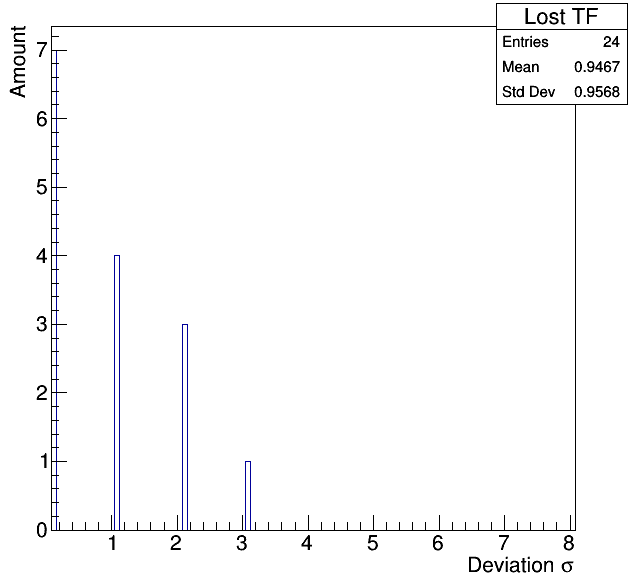
\includegraphics[scale=0.5]{./graphics/ex2_histogram.png}
	\caption{Histogram of the TF lost for ticktime 5}
	\label{Ex2Histogram}
\end{figure}

\newpage

\section{Ex.3 2 FLPs 12 EPNs}
\textbf{Ticktime influence on the Blacklist algorithm with all but one-fail over with random sample size.}
\\~\\
Compliant with the previous results, the TF loss to ticktime ratio rises in a linear line, with no absurdities along the way. The amounts are also negligibly different to the previous results. Results can be seen in table ~\ref{table:Ex3MitchResults} and table ~\ref{table:Ex3HeikoResults}. A histogram for ticktime 5 can be seen at ~\ref{fig:Ex3Histogram}. It shows a standard deviation of 1.569 for all the TFs lost in the entire run. 

\begin{table}[htb]
\resizebox{\textwidth}{!}{\begin{tabular}{| p{0.1\linewidth} | >{\centering}m{0.7cm} | >{\centering}m{0.7cm} | >{\centering}m{0.7cm} | >{\centering}m{0.7cm} | >{\centering}m{0.7cm} | >{\centering}m{0.7cm} | >{\centering}m{0.7cm} | >{\centering}m{0.7cm} | >{\centering}m{0.7cm} | >{\centering}m{0.7cm} | >{\centering}m{0.7cm} |}
\hline
Lost EPNs & 1 EPN & 2 EPNs & 3 EPNs & 4 EPNs & 5 EPNs & 6 EPNs & 7 EPNs & 8 EPNs & 9 EPNs & 10 EPNs & 11 EPNs \tabularnewline \hline
Ticktime &&&&&&&&&&& \tabularnewline \hline
5 &  &  &  &  &  &  &  &  &  &  &  \tabularnewline \hline
10 & 2 & 2 & 3 & 3 & 3 & 3 & 3 & 3 & 4 & 5 & 7 \tabularnewline \hline
15 & 3 & 3 & 3 & 3 & 4 & 4 & 4 & 5 & 6 & 7 & 9 \tabularnewline \hline
20 & 3 & 3 & 4 & 4 & 4 & 4 & 5 & 6 & 6 & 8 & 12 \tabularnewline \hline
25 & 4 & 4 & 4 & 4 & 4 & 5 & 6 & 7 & 8 & 10 & 13 \tabularnewline \hline
\end{tabular}}
\caption{Cumulative lost TFs by ticktime/EPN ratio with a random sample size for the Blacklist algorithm}
\label{table:Ex3MitchResults}
\end{table}

\begin{table}[htb]
\resizebox{\textwidth}{!}{\begin{tabular}{| p{0.1\linewidth} | >{\centering}m{0.7cm} | >{\centering}m{0.7cm} | >{\centering}m{0.7cm} | >{\centering}m{0.7cm} | >{\centering}m{0.7cm} | >{\centering}m{0.7cm} | >{\centering}m{0.7cm} | >{\centering}m{0.7cm} | >{\centering}m{0.7cm} | >{\centering}m{0.7cm} | >{\centering}m{0.7cm} |}
\hline
Lost EPNs & 1 EPN & 2 EPNs & 3 EPNs & 4 EPNs & 5 EPNs & 6 EPNs & 7 EPNs & 8 EPNs & 9 EPNs & 10 EPNs & 11 EPNs \tabularnewline \hline
Ticktime &&&&&&&&&&& \tabularnewline \hline
5 & 1 & 2 & 2 & 2 & 2 & 3 & 3 & 3 & 3 & 4 & 4 \tabularnewline \hline
10 & 1 & 3 & 3 & 3 & 3 & 3 & 3 & 4 & 4 & 5 & 6 \tabularnewline \hline
15 & 11 & 3 & 3 & 3 & 3 & 3 & 4 & 4 & 5 & 6 & 7 \tabularnewline \hline
20 & 10 & 3 & 3 & 3 & 4 & 4 & 4 & 5 & 6 & 7 & 9 \tabularnewline \hline
25 & 13 & 3 & 4 & 4 & 4 & 4 & 5 & 5 & 7 & 8 & 10 \tabularnewline \hline
\end{tabular}}
\caption{Cumulative TF data loss across events with the Blacklist algorithm and a random sample size (van der Heijden, 2018, p. 40)} 
\label{table:Ex3HeikoResults}
\end{table}

\begin{figure}
	\centering
	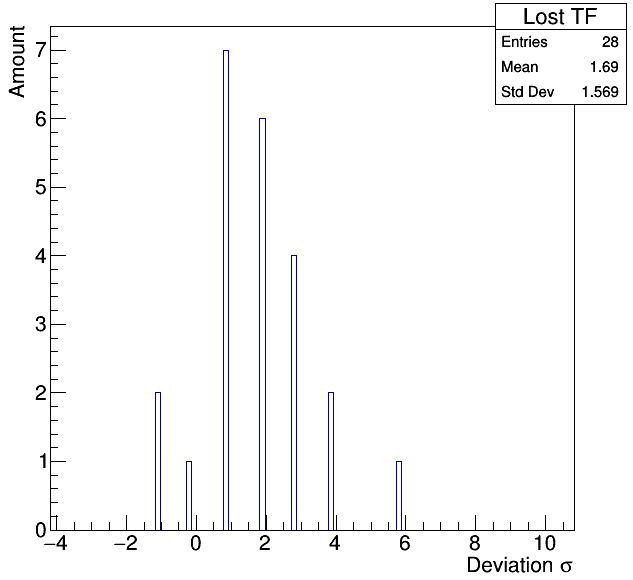
\includegraphics[scale=0.5]{./graphics/ex3_histogram.png}
	\caption{Histogram of the TF loss for ticktime 5}
	\label{fig:Ex3Histogram}
\end{figure}

\newpage

%\section{Ex.1 3 FLPs 18 EPNs}
%\textbf{Ticktime influence on the Blacklist algorithm with one fail-over.}
%\\~\\

%\section{Ex.2 3 FLPs 18 EPNs}
%\textbf{Ticktime influence on the Blacklist algorithm with all but one fail-over.}
%\\~\\

%\section{Ex.3 3 FLPs 18 EPNs}
%\textbf{Ticktime influence on the Blacklist algorithm with all but one-fail over with random sample size.}
%\\~\\

%\section{Ex.1 4 FLPs 24 EPNs}
%\textbf{Ticktime influence on the Blacklist algorithm with one fail-over.}
%\\~\\

%\section{Ex.2 4 FLPs 24 EPNs}
%\textbf{Ticktime influence on the Blacklist algorithm with all but one fail-over.}
%\\~\\

%\section{Ex.3 4 FLPs 24 EPNs}
%\textbf{Ticktime influence on the Blacklist algorithm with all but one fail-over with random sample size.}
%\\~\\

%\section{Ex.4 4 FLPs 24 EPNs}
%\textbf{Ticktime influence on the Blacklist algorithm with all but one fial-over at once.}

\section{Analysis}
\subsection{Comparison to the previous experiment}
Looking at the data from experiment two and three, the difference is almost negligible. For the first EPN that crashes there is a 1-2 difference of TFs lost, and for the last EPN there is 2-3 difference. The difference is mainly from the first experiment. It seems that the new cluster is a bit less functional on uneven ticktimes. 
%\subsection{Increasing the numbers of FLPs and EPNs}
